\documentclass[man,noapacite]{apa2}
\usepackage{amsmath}
\usepackage{booktabs}
\usepackage{apacite2}
\usepackage{fullpage,rotating}
\usepackage{pslatex}
\usepackage{amssymb}
\usepackage{setspace}

\title{\vspace{-16ex} Rational speech act models of pragmatic reasoning in reference games}

\sixauthors{Michael C. Frank}{Andr\'es G\'omez Emilsson}{Alex J. Stiller}{Benjamin Gittelson}{Christopher G. Potts}{Noah D. Goodman}
\sixaffiliations{Department of Psychology, Stanford University}{Department of Psychology, Stanford University}{Department of Linguistics, University of California, San Diego}{Department of Linguistics, Columbia University}{Department of Linguistics, Stanford University}{Department of Psychology, Stanford University}

\shorttitle{Rational speech act models}
\rightheader{Rational speech act models}


\newcommand{\argmax}{\operatornamewithlimits{argmax}}

% EXPERIMENT COUNTER
\newcounter{Experiment}
\setcounter{Experiment}{0}
\newcommand{\expt}[1]{\protect\refstepcounter{Experiment}\arabic{Experiment}\label{#1}}
\newcommand{\exptref}[1]{Experiment\,\ref{#1}}
\newcommand{\exptrefrange}[2]{Experiments\,\ref{#1}--\ref{#2}}
\newcommand{\exptrefnoexpt}[1]{\ref{#1}}


% SECTION REFERENCES
\newcommand{\secref}[1]{Section\,\ref{#1}}
% \newcommand{\secref}[1]{section\,\ref{#1}}
% \newcommand{\dashsecref}[2]{sections\,\ref{#1}--\ref{#2}}

\acknowledgements{\singlespace Thanks to Avery Katko and Paul Mains for assistance in data collection and design for \exptrefrange{exp:seqs-1}{exp:prod-2seq}. Thanks to Roger Levy for much valuable discussion and the design of the ``odd man out'' stimulus. Thanks to Allison Kraus for designing the stimuli used here.  Some of these ideas and experimental designs were presented in substantially different form in \citeA{stiller2011}; data from \exptref{exp:levels-level} were presented in \citeA{vogel2014}. We gratefully acknowledge funding from ONR and the Merck Family Foundation. Please address correspondence to Michael C. Frank, Department of Psychology, Stanford University, 450 Serra Mall (Jordan Hall), Stanford, CA, 94305, tel: (650) 724-4003, email:{\texttt mcfrank@stanford.edu}.

~\\
}


\abstract{Human communication is almost always underspecified, but it typically takes place in a context where otherwise ambiguous messages can be decoded. A key part of this process of pragmatic disambiguation comes from reasoning about the possible alternative messages that could have been said in that context. Consolidating previous modeling work, we describe this process of recursive reasoning---in which listeners reason about speakers and vice versa---through a ``rational speech act'' (RSA) model. We then systematically test the parameters and design decisions of this model through a series of more than 20 experiments using simple one-shot reference-resolution games. Such games present a valuable and tractable microcosm for studying broader questions about communication in context, and human behavior within them is well-described within the dynamics of the RSA model.}

\begin{document}
\maketitle                            

\section{Introduction}

Human communication is astonishingly flexible and efficient. Between two people who know each other well, a single word, look, or gesture can convey volumes \cite{sperber1986,clark1996}. Even two people who barely know one another can rapidly leverage their shared vocabulary to create new, economical ways of communicating about novel situations \cite{brennan1996,clark1991}. These successes are all the more impressive considering the systematic issues of vagueness and ambiguity in natural language \cite{keefe1997,wasow2005}. How do we use such slippery means to produce such concrete results? 

\citeA{grice1975} provided a critical insight into this problem: listeners could reason about speakers' goals in choosing a particular form for their communication. By assuming that speakers were attempting to be cooperative in their communicative, listeners could then infer the most likely intended goal that would have given rise to that form, given the current circumstances. This proposal allowed the separation of semantic content---those aspects of meaning that are invariant across contexts---from pragmatic content---those aspects of meaning that rely on contextual inferences about speaker intentions. 

Although many subsequent analysts have attempted to refine Grice's original proposal or even to reject substantial elements, the semantics/pragmatics distinction has been critical for progress in understanding language comprehension. Nevertheless, because of the difficulties of formalizing notions like context and social goal inference, pragmatics has often remained a ``wastebasket'' for phenomena that are difficult to explain under formal theories of syntax or semantics \cite{bar-hillel1971}. This dismissal of pragmatics is regrettable because of the importance and richness of pragmatic phenomena. In some substantial sense, what linguists call ``pragmatics'' is what language users experience as the use of language in their everyday interpersonal communication---the reality of how context alters interpretation. Thus, an important goal for research in linguistics and the psychology of language is the development of formal tools for understanding pragmatic inferences and bringing them under experimental control. 

In this article, we report on a formal framework for understanding pragmatics, known as the ``rational speech act'' (RSA) framework \cite<originally introduced in>{frank2012,goodman2013}. This framework builds on Grice's initial insight and combines it with tools from Bayesian cognitive modeling \cite{tenenbaum2011}. The result is a set of tools for a quantitative understanding of the kind of social goal inference that Grice initially described. In the remainder of this introduction, we provide a relatively brief survey of qualitative frameworks for pragmatic reasoning, and then discuss quantitative progress in quantitative models of pragmatics. We then summarize the plan for the rest of the article.

\subsection{Qualitative models of pragmatic reasoning}

Grice

Horn

Levinson

Sperber and Wilson

Chierchia et al. 

\subsection{Quantitative models of pragmatic reasoning}

Early work, hobbes, etc. 

referring expression generation

percy liang

Game-theoretic approaches - parikh, van rooj, Franke, Jaeger

RSA models - antecedents in social reasoning models \cite{baker2009}

\subsection{The current work}

The current work has two interlocking goals. The first goal is empirical: via a sequence of large-scale, web-based experiments, we provide strong evidence that one-shot reference games provide a flexible and precise tool for studying quantitative patterns of human behavior. The second goal is formal: we provide a more comprehensive presentation of ``rational speech act'' (RSA) models of pragmatic reasoning and show that this framework captures many of the patterns of performance we observed in our experiments. Taken together, this body of work suggests that the RSA model provides a powerful set of tools for studying human pragmatic reasoning in quantitative detail. 

Our experiments are listed in Table \ref{tab:expts}; they are broken into three sequences. The first of these (``Preliminaries,'' Section \ref{sec:prelims}) explores our primary experimental paradigm, one-shot reference games, providing experimental evidence that minor design choices do not account for the pattern of data we observe. The second section (``Priors,'' Section \ref{sec:prior}) tests the role of prior expectations in reference game behavior. The third (``Levels,'' Section \ref{sec:levels}) tests the level of recursion that speakers reason to and provides further data on the relationship between prior and posterior measurements. 
% The fourth (``Sequences,'' Section \ref{sec:seqs}) takes a first step towards exploring sequential effects in pragmatic reasoning and whether these can scaffold more deeply referential expressions. The fifth and final section (``Production,'' Section \ref{sec:prod}) discusses speaker behavior in reference games and shows that it is sensitive to the costs of language production. 

Our plan is as follows. We first present formal details of the RSA model. We next move to our experimental presentation. We then examine the fit of RSA models to our data. To conclude, we discuss limitations and future directions for RSA modeling, as well implications of this work for the study of pragmatics more broadly. 

%%% Local Variables: 
%%% TeX-master: "pragmods"
%%% End:



\section{Formal Framework}
\label{sec:models}

In this section, we describe formal details of the ``rational speech act'' model. As described above, this model has been presented previously \cite{frank2012,goodman2013}. Our goal here is to provide a more comprehensive formal presentation. This presentation allows us to highlight choice-points in the model that we test below; in addition, it illuminates parallels and differences with other formal models in this space (specific comparisons are given in Appendix \ref{app:equivalences}).

% We introduce a notation for signaling games and other recursive reasoning problems \cite{golland2010,franke2012,frank2012,goodman2013}. This notation system allows us to define a set of recursive models; we show that a set of recent systems for pragmatic reasoning can be written within this system. As a consequence, they are equivalent to one another modulo three design decisions: 


\subsection{Preliminaries}

A reference game under our definition is a game in which a speaker $S$ and listener $L$ collaborate in a context $C$ to identify a particular object in the context, known as the speaker's intended referent $r_S \in C$. The game has two parts. First the speaker chooses an utterance $w$ based on vocabulary $V$; this process can be as simple as selection from a list or as complex as generation from a grammar. Next the listener guesses a referent $r_L \in C$ after hearing $w$. The game is won if $r_S=r_L$.

There is a ``contextual salience'' distribution $\sigma$ over the objects ${o_1 ... o_n} \in C$, which is mutually known to both speaker and hearer. This distribution picks out those objects in the context which are more or less likely to be talked about, either because of their intrinsic perceptual or conceptual noteworthiness, or because of some prior history between speaker and listener (e.g. one object having been talked about previously). 

There is also a mutually-known semantics for the vocabulary of possible words (messages) $w$ that a speaker can send.  Each message can be described as a Kronecker $\delta$ function that applies to referents and returns 1 if the message is true of that referent, 0 otherwise. 

\subsection{The model}

We define the RSA model in terms of two agents, a listener $L$ and a speaker $S$. Their goals are to reason about one another so that they are able to transmit information efficiently. $L$ reasons abut what word $S$ would have said to describe a particular referent; $S$ reasons about what interpretation $L$ would give to a particular message. Each of these agents uses Bayesian inference to reason about the other's likely actions. 

So we can define:

\begin{equation}
  \begin{array}{r@{}l}
    \label{eq:agents}
    P_L(r_S | w, C) & \propto P_S (w | r_S, C) P(r_S)\\
    P_S(w | r, C) & \propto P_L (r_S | w, C)  
  \end{array}
\end{equation}

\noindent where $P(r_S)$ is a prior distribution over referents, which we discuss extensively below. In principle, we could also add a prior on words, $P(w)$, but for simplicity here we assume that $P(w) \propto 1$ and do not discuss it further. 

The two agents in Equation \ref{eq:agents} are defined recursively and so individual probabilities are undefined unless the recursion ends. Thus, we define a further agent, $L_0$, the ``literal listener,'' who grounds the recursion:

\begin{equation}
P_{L_0} (r_S | w, C) \propto \begin{cases} \frac{1}{\sum_{r \in C} \delta_w(r)} &\mbox{if } \delta_w(r_s) = 1 \\ 
0 & \mbox{otherwise.} \end{cases} 
\end{equation}

\noindent In other words, agent $L_0$ simply chooses uniformly between available referents that are consistent with $w$. 

With these agents defined, we can then imagine variations on this model where $L$ reasons about $S$, who in turn reasons about $L_0$. 

See Appendix \ref{app:alternative}

\subsection{Choice-points}

\begin{enumerate}
\item The depth of the recursion between speaker and listener,
\item Whether the recursion starts with speaker or listener,
\item The decision rule chosen by speaker and listener (soft vs. hard maximization), and 
\item Whether the model includes a term indicating the prior probability of a referent being talked about.
\end{enumerate}

\noindent We show equivalences of various special cases of this notation to the systems described in these prior reports.

\subsection{An example}

% \begin{figure}[t]
%   \begin{center} 
%     \includegraphics[width=4.5in]{figures/bugs.jpg} 
%     \caption{\label{fig:ex} An example stimulus for our 3 objects, 3 features experiment. Inferring that ``tail'' referred to C is a depth-0 computation, inferring that ``feet'' referred to A is a depth-1 computation, and inferring that ``horns'' referred to B is a depth-2 computation.} 
%   \end{center} 
% \end{figure}

We work through an example computation on the stimulus shown in Figure \ref{fig:ex}, using the J\"ager \cite{jaegerinpress} version of the model described above (for simplicity and finite convergence): $L^*(S^*(L^*(S(C^T))))$. The object by feature matrix $C$ has as its columns the messages ``tail,'' ``horns,'' and ``feet'' and the objects A, B, and C as its rows.:

\begin{equation}
C= \left(
    \begin{array}{ccc}
      0 & 0 & 1 \\
      0 & 1 & 1\\
      1 & 1 & 0 
    \end{array} 
  \right)
\end{equation}

The corresponding speaker matrix $S(C^T)$ is inverted, with messages as rows and objects as columns: 

\begin{equation}
E = \left(
    \begin{array}{ccc}
      0 & 0 & 1 \\
      0 & .5 & .5\\
      .5 & .5 & 0 
    \end{array} 
  \right)
\end{equation}

It is already clear that ``tail'' is true only of object C, thus the interpretation of ``tail'' reaches depth 0. Now we perform a set of renormalizations to lead to the next level of recursion:

\begin{equation}
L^*(S(C^T)) = \left(
    \begin{array}{ccc}
      0 & 0 & 1 \\
      0 & .5 & .5\\
      1 & 0 & 0 
    \end{array} 
  \right)
\end{equation}

Now, at depth 1, the message ``feet'' is found to refer to object A. A final round of recursion leads to depth 2, where ``horns'' is found to refer to object B:

\begin{equation}
L^*(S^*(L^*(S(C^T)))) = \left(
    \begin{array}{ccc}
      0 & 0 & 1 \\
      0 & 1 & 0\\
      1 & 0 & 0 
    \end{array} 
  \right)
\end{equation}

We now say that the model has ``converged''---that is, further iteration will not lead to changes in state.

\subsection{Status of the model}

%%% Local Variables: 
%%% TeX-master: "pragmods"
%%% End:


\section{General Experimental Methods}

This section describes the methods used in the experiments reported below. Our goal was to create a general method for measuring pragmatic inferences in simple reference games. Our taking-off point is two previous studies in which simple feature-based displays allowed measurement of pragmatic reasoning in grounded contexts \cite{frank2012,stiller2014}. In what follows we describe some of the general features of these displays and the experiments that use them.
% In the experiments that follow we attempt to demonstrate that these signaling games provide a useful tool for measuring pragmatic reasoning. 

\subsection{Participants}

One challenge of pragmatic communication experiments is that repeated communication within a signaling game is very likely to influence responding \cite<e.g.,>{brennan1996}. For this reason, we adopted a massively between-subjects approach, where each participant answered exactly one relevant question.

We adopted a general standard of 50 independent participants per cell, based on the tradeoff between cost and the desired precision of measurements. With samples of N=50 participants making binary decisions, we could assume 95\% confidence intervals with width .24 at their widest; doubling the sample size to N=100 per cell would only reduce width to .18. While not every experiment reflects this precise standard due to idiosyncrasies of recruitment exclusion, we have tried to maintain approximately this standard throughout. 

All of the experiments described here were run on Amazon's Mechanical Turk crowdsourcing service, between Fall 2013 and Spring of 2015. In general, each experiment was run as an independent human intelligence task (HIT); a few were posted as multiple hits for convenience or due to experimenter error. In all cases, we remove duplicated workers from the samples, so that data in each experiment represent a set of unique judgments by distinct participants. 

In addition to excluding duplicated participants, we also excluded participants who failed manipulation checks (see below). Table \ref{tab:expts} gives details of participants for each experiment. 

\subsection{Stimuli}

We created a set of six base domains that had features that could easily be added independently: faces (pictured in Figure \ref{fig:ex}), boats, pizzas, sundaes, snowmen, and christmas trees. We created slightly different versions of each base so that they would appear to be unique (e.g., by varying the proportions or color tone of the face). We then were able to add features to each of these programmatically (with most experiments using two features but some using three). Faces were supplemented with hats, glasses, and mustaches; boats had motors, sails, and cabins; pizzas had olives, peppers, and mushrooms; sundaes had whipped cream, chocolate, and cherries on top; snowmen had mittens, hats, and scarves; and christmas trees had lights, ornaments, and stars on top.

\subsection{Procedure}

Participants viewed the experiment within a browser window. The first screen of the experiment presented a basic description of the paradigm and asked for informed consent. The second screen of the experiment presented the interlocutor, Bob (a cartoon picture of a man), and noted that he liked to do activities with the base item (e.g., visit friends or sail boats). In experiments with familiarization stimuli (e.g., \exptref{exp:prior-baserate}), nine familiarization images were presented on this screen. 

The third screen was the key screen: it presented the experimental stimulus (a set of base items augmented with features, representing the signaling game of interest) at the top of the screen. Below each stimulus a letter was displayed. From left to right: A, B and C. In all experiments except for \exptref{exp:prelims-mc}, two manipulation check questions were asked directly below the display using text entry boxes (e.g. ``how many boats have cabins?''). Below this was the prompt, e.g. ``Bob can only say one word to communicate with you and he says: {\it glasses}. Click below on the option that represents the friend that you think Bob is talking about.'' Below this was a set of buttons labeled A, B and C for the participant to indicate which of the three options they thought the speaker was referring to. A final screen asked participants the following: ``Who did you meet in this survey?'',  ``What was this survey about?'' and ``Any other comments for us?'' Optionally, participants could also provide their age and gender, but finishing the experiment was not contingent on doing this.

Note that in the first set of experiments, we manipulate a number of these experimental choices, including the dependent variable, the use of the manipulation check, and the linguistic framing of Bob's utterance. Our description here reflects the defaults used in the majority of the experiments we report. 



% Minor stuff:

% Prelims measures has four items

% Size and sequence have no manipulation check 

%%% Local Variables: 
%%% TeX-master: "pragmods"
%%% End:


\begin{table}
\caption{\label{tab:expts} Outline of the experiments reported here.}
\begin{tabular}{cllllll}
\hline
Expt. \# & Sequence & Experiment & $N_{total}$ & $N_{include}$ & Summary \\
\hline
\expt{exp:prelims-dv} & Prelims & Dependent variable & 689 & 554 & Forced choice yields best DV \\
\expt{exp:prelims-mc} & & Manipulation check & 580 & 513 & Modest increase in inference for MC \\
\expt{exp:prelims-frame} & & Linguistic frame & 100  & 89 & No difference\\
\expt{exp:prior-frame} & Prior & Elicitation frame & 200 & 175 & No difference \\
\expt{exp:prior-baserate} &  & Base rate & 800 & 488 & Base rate affects inference \\
\expt{exp:prior-valence} &  & Linguistic framing & 550 & 502 & Linguistic valence affects inference\\
\expt{exp:prior-color} &  & Perceptual salience & 300 & 267 & \\
\expt{exp:levels-level} & Levels & Level of inference & 520 & 453 & Level 2 difficult for participants \\
% \expt{exp:levels-prior} &    & Levels prior & & CHECK  & \\
\expt{exp:levels-twins}  &    & Twins & 120 & 106  & Hard to get non-literal readings\\
\expt{exp:levels-oddman} &    & Oddman & 200 & 182  & Hard to get non-literal readings\\
% \expt{exp:levels-twinsprior} &    & Twins prior & & CHECK \\
% \expt{exp:levels-oddmanprior}&    & Oddman prior & & CHECK \\
\expt{exp:levels-dists} &  & Distractors & 1300 & 1224 & Model captures matrix layout\\
% \expt{exp:size-distsprior} &  & Distractors prior & TODO & & \\
\expt{exp:seqs-1} & Sequences & Level 1 & 200 & 191 & Limited sequential effect, no transfer \\
\expt{exp:seqs-1x3} & & Level 1 x3 & 200 & 193 & No repetion effects \\
\expt{exp:seqs-2} & & Level 2 & 100 & 93 & Strong sequence effect for L2 \\
\expt{exp:prod-1} & Production & Level 1 & 450 & 383 & Cost affects overspecification\\
\expt{exp:prod-1seq} & & Level 1 sequential & 453 & 394 & Production increases L1 inference\\
\expt{exp:prod-2seq} & & Level 2 sequential & 450 & 389 & Production doesn't increase L2 inference\\
\hline
\end{tabular}
\end{table}

\section{Methodological preliminaries}
\label{sec:prelims}

Our first set of experiments, \exptrefrange{exp:prelims-dv}{exp:prelims-frame}, establish the simple reference games in Figure \ref{fig:ex} as a viable method, testing the replicability of judgments in this paradigm and examining particular experimental decisions. 

\begin{figure}[t]
  \centering
  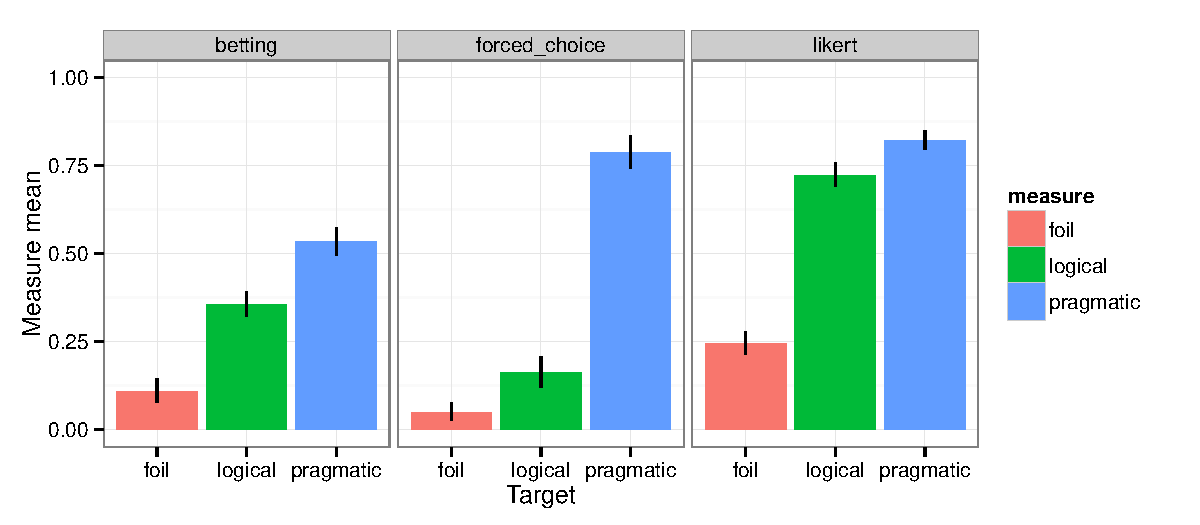
\includegraphics[width=6in]{../plots/1-prelims-dv.pdf}
  \caption{\label{fig:prelims-dv} Data from \exptref{exp:prelims-dv}. Each panel shows results from a different dependent variable (normalized for simplicity into the interval [0,1]. The three columns show results for the foil (e.g., face with nothing), logical (e.g., face with hat and glasses), and pragmatic (face with only glasses) targets. Error bars show 95\% confidence intervals, computed by non-parametric bootstrap.}
\end{figure}

Experiment \exptref{exp:prelims-dv} explored the use of different dependent variables. We considered a betting measure, in which participants were instructed to allocate \$100 across the three targets, as in \citeA{frank2012}; a 7-point Likert scale, as in \citeA{goodman2013}; and a simple three-alternative forced choice measure.\footnote{As this experiment was one of our first, we used only four of our six stimulus items: faces, boats, snowmen, and sundaes.} Figure \ref{fig:prelims-dv} shows results from each. With all three dependent variables, the pragmatic target was chosen more than the logical target, but this result was strongest for the forced choice, with 79\% of participants choosing the pragmatic target. Both the Likert and betting measures afforded the possibility of ``hedging'' by allocating equal bets or ratings to the pragmatic and logical targets. Conservative participants took advantage of this possibility very frequently, betting equal amounts on the logical and pragmatic targets 43\% of the time and using equal Likert ratings 46\% of the time. In contrast, the forced-choice did not allow this kind of hedging; thus, we adopt it in our further experiments.  

Experiment \exptref{exp:prelims-mc} was designed to ensure that the presence of the manipulation check--asking participants to count how many of each feature was present---did not induce a task demand that changed the magnitude of pragmatic responding. We saw 83\% pragmatic responding in the manipulation check condition and 77\% pragmatic responding in a matched condition with no manipulation check. Because of the high power of this experiment ($N_{include}$ = 513), the difference between conditions was statistically significant ($\chi^2(2) = 6.97,~p = .03$). Nevertheless, the modest (6\%) difference between conditions suggests that the manipulation check does not \emph{create} the pragmatic effect, though it may heighten participants' attentions to the different distributions of the two features, leading to slightly more pragmatic responding. We continue to use the manipulation check as an exclusion criterion in further experiments. 

Experiment \exptref{exp:prelims-frame} was designed to test the particular linguistic framing we used, in particular contrasting the presentation of the target word (e.g. ``glasses'') as part of a phrase, ``Bob says: 'My friend has glasses.' '' and a presentation of the target word with the framing that the speaker is can only say a single word (described above in the General Methods). The ``one word'' framing produced 80\% pragmatic responses, while the ``My friend has glasses'' framing produced 82\% pragmatic responses. These frames did not differ significantly from one another in the distribution of responses they produced ($\chi^2(2) = 2.54,~p = .28$). Except where noted below, we adopt the one-word framing. 

In sum, these findings suggest that aspects of the experimental presentation and dependent variable have some effects on the magnitude of the pragmatic effect we observed. Nevertheless, the existence of the effect is quite robust to these variations. 


\section{Measuring and manipulating prior expectations}

Our second set of experiments, \exptrefrange{exp:prior-frame}{exp:prior-salience}, examine the role of prior expectations in the RSA model's pragmatic computations. These experiments serve two goals. First, they create a set of quantitative measurements of prior expectations combined with listener inferences; these measurements can be used for model comparison and assessment, a topic that we return to in \secref{sec:modelcomp}. Second, they allow causal inferences about the role of the prior in participants' pragmatic inferences. While \citeA{frank2012} \emph{measured} prior expectations and showed that they improved model fit, that work did not \emph{manipulate} prior expectations, so it was in principle possible that improvements in model fit did not result from a causal role played by prior expectations. We address this issue in the studies below. We begin by comparing methods for eliciting prior expectations (\exptref{exp:prior-frame}). We then investigate three ways of manipulating prior expectations: via base-rates (\exptref{exp:prior-baserate}), via linguistic valence (\exptref{exp:prior-valence}), and via perceptual salience (\exptref{exp:prior-salience}). 

It is not immediately clear what the best way is to measure prior expectations for purposes of communication. One particular conceptual issue seems important, though: does the term $p(r_s)$ refer to a prior over \emph{reference}, that is, over things that a speaker would talk about? Or does it instead represent a prior over \emph{actions}, that is, over the things that a speaker would do? This is a fairly deep philosophical issue; but it also has important empirical consequences for our current project. If these two kinds of priors differ substantially, then our estimates of $p(r_S)$ might lead to incorrect conclusions. In particular, \citeA{frank2012} introduced a method in which priors were measured identically to listener judgements, with the exception that participants in the prior measurement condition were not given any linguistic information. They were told that the speaker could utter one word to signal their target referent, but that they (the listener) hadn't heard it. This method yielded reliable measurements, but presupposed that the prior was over reference, rather than action. 


\begin{figure}[t]
  \centering
  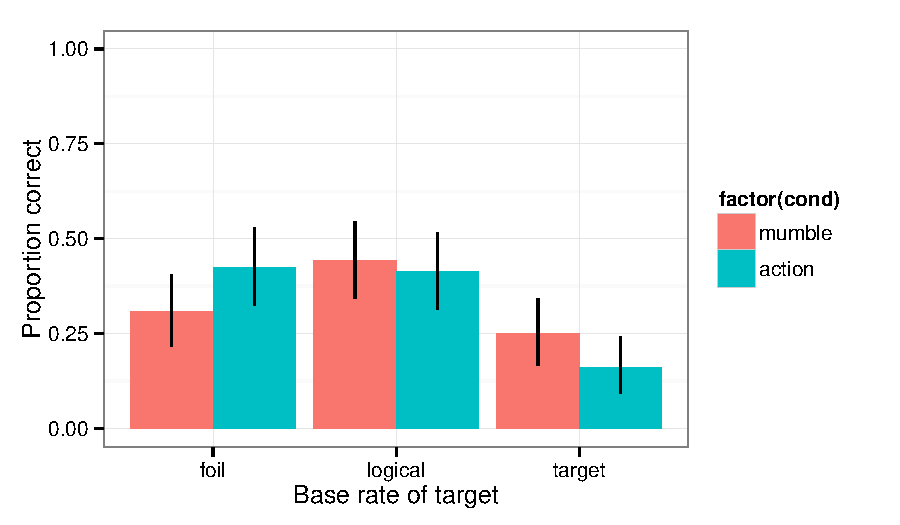
\includegraphics[width=5in]{../plots/2-prior-frame.pdf}
  \caption{\label{fig:prelims-dv} Data from \exptref{exp:prior-frame}. Colors indicate different methods for eliciting prior expectations.}
\end{figure}

In \exptref{exp:prior-frame}, we compared prior elicitation methods. We presented participants with the same canonical display we had used in the prior experiments, but asked them one of two prior questions. The reference prior method was based on \citeA{frank2012}, where the participant was told that ``Bob can say one word'' but the word was presented as ``mumblemumble (you didn't hear what he said).'' The action prior method consisted of simply asking, e.g. ``Which friend do you think Bob will visit next?'' The distribution of responses did not differ between the two questions ($\chi^2(2) = 3.45,~p = .18$, Figure \ref{fig:prior-frame}). Overall, participants showed a tendency to choose the logical target (e.g., face with both hat and glasses) most, the foil at intermediate rates, and the pragmatic target relatively less. While this experiment is not decisive regarding the underlying philosophical issue of what kinds of expectations the prior actually tracks, we put aside this issue for the time being and adopt the mumble prior elicitation method for subsequent experiments (as the choice does not appear critical for our purposes).

\begin{figure}[t]
  \centering
  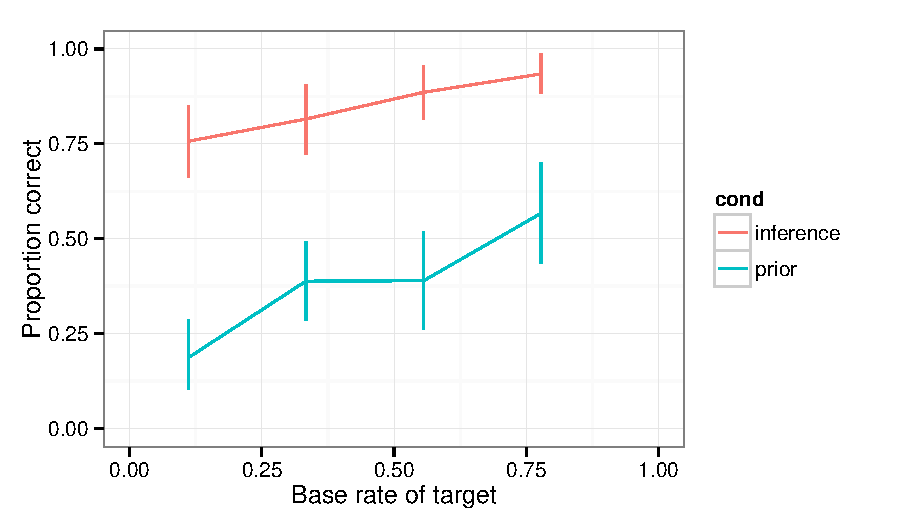
\includegraphics[width=5in]{../plots/2-prior-baserates.pdf}
  \caption{\label{fig:prior-baserate} Data from \exptref{exp:prior-baserates} from prior elicitation and inference conditions. Horizontal axis shows the proportion of familiarization trials that showed the target.}
\end{figure}

In \exptref{expt:baserate}, we attempted to manipulate participants' prior expectations about reference via a manipulation of the base rate of the interlocutor's actions.\footnote{This experiment is conceptually similar to a base-rate manipulation reported in \citeA{stiller2011}. Note however that the manipulation in that experiment uses a different display, one more similar to those used in \exptref{exp:levels-level}.} Prior to showing the target inference, we exposed participants to evidence about the habits of the interlocutor (Bob). The familiarization screen in this experiment stated (for example, in the case of the face stimulus) that Bob visited a friend every week; it then invited the participant to click on nine boxes to uncover the nine friends that Bob had visited most recently. Across four base rate conditions, we manipulated how many of these boxes contained the pragmatic target (e.g., the face with glasses and no hat). One of the boxes always contained the foil (no glasses or hat) and another contained the logical target (hat and glasses). Then the other boxes contained either the pragmatic or the logical target. The four conditions were created such that 1/9, 3/9, 5/9, and 7/9 boxes showed the pragmatic target. 

Figure \ref{fig:prior-baserate} shows the results of this manipulation.\footnote{This experiment had unusually high rates of exclusion due to participants' confusion about whether they should report  familiarization frequencies for the manipulation check. We maintain our strict inclusion criterion here but note that the results are largely unchanged if we include these participants.}  The base rate had a strong effect on the prior elicitation, but it also boosted levels of pragmatic inferences. To quantify these effects preliminary to model fitting, we used a logistic regression model (no hierarchical model was warranted because judgments are from independent participants). This model showed highly significant effects of base rate ($\beta = .27,~p = .004$) and condition  (with prior as the dummy-coded predictor, $\beta = -.57,~p < .0001$), as well as a marginal interaction of the two  ($\beta = .29,~p = .06$). Critically, the main effect of base rate remained reliable in a similar logistic regression for just the inference trials ($\beta = .28,~p = .0001$), indicating a highly reliable (and graded) effect of the base-rate manipulation on the strength of the pragmatic inference.

Our next experiment, \exptref{exp:prior-valence}, investigated 


Our final experiment in this sequence, \exptref{exp:prior-salience}, investigated the role of salience 


In sum, these experiments show strong evidence that a variety of manipulations can affect prior expectations about reference.  

\section{Levels of recursion and limits on human reasoning}
\label{sec:levels}

In our next set of experiments, \exptrefrange{exp:levels-levels}{exp:levels-size}, we continue to 

% \section{Scalability with matrix size}
\label{sec:size}



\section{Sequential reasoning in reference games}
\label{sec:seqs}



\section{Speaker behavior in reference games}
\label{sec:prod}



\section{Model fits and model comparison}
\label{sec:models}

In the experiments reported above, we see strong evidence that participants are engaging in reasoning that goes beyond the simple semantic interpretation of messages. Instead, they appear to be making inferences about reference in context that have the character of pragmatic reasoning---considering inferential alternatives that a speaker could have said. In this section, we test the ability of the RSA model to describe human behavior in these experiments. 

We are well aware of the difficulties surrounding reasoning from a good fit alone \cite{roberts2000}. In a nutshell, any model must both show that it \emph{can} predict the data that actually occurred and \emph{cannot} predict the data that did not occur. The flexibility of the theory is thus of critical importance in understanding its performance. The RSA model as stated here and earlier contains a relatively small number of parameters, however: primarily $n$ (the depth of recursion) and $\alpha$, the greed parameter in the choice rule. 

 \begin{figure}[t]
  \centering
  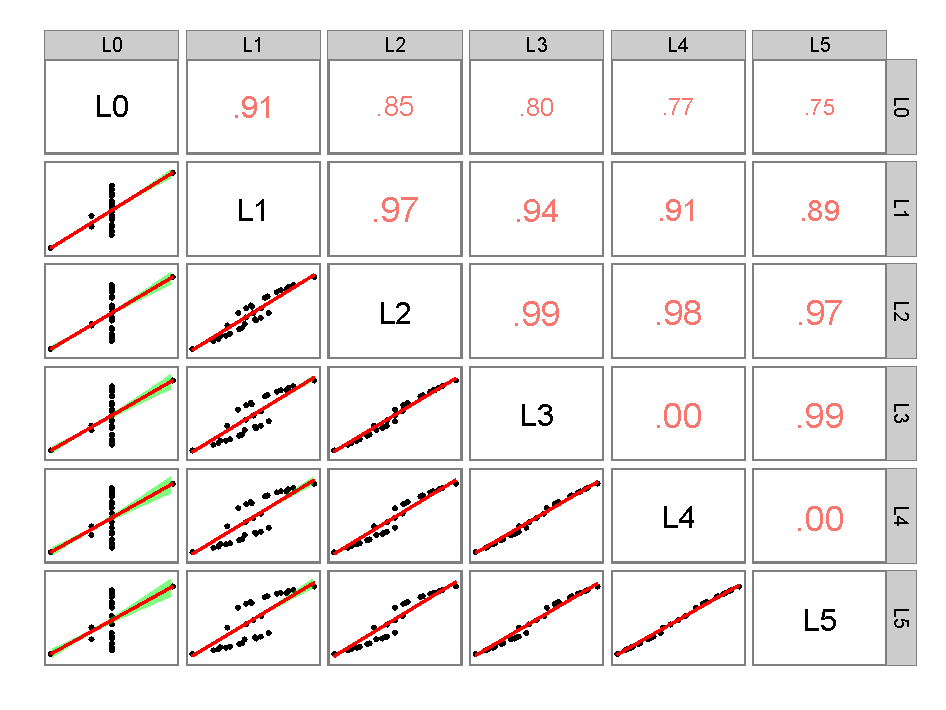
\includegraphics[width=6in]{../plots/models-2.pdf}
  \caption{\label{fig:models-2} Model identifiability simulation results. Each plot on the lower triangle shows model predictions for one model plotted by predictions for another. Each dot is an experimental condition, with trend lines showing simple linear regression with 95\% confidence intervals. Each plot on the upper triangle shows the pearson correlation value between those two models. Models with higher levels of recursion are very difficult to distinguish from one another.}
\end{figure}


 \begin{figure}[t]
  \centering
  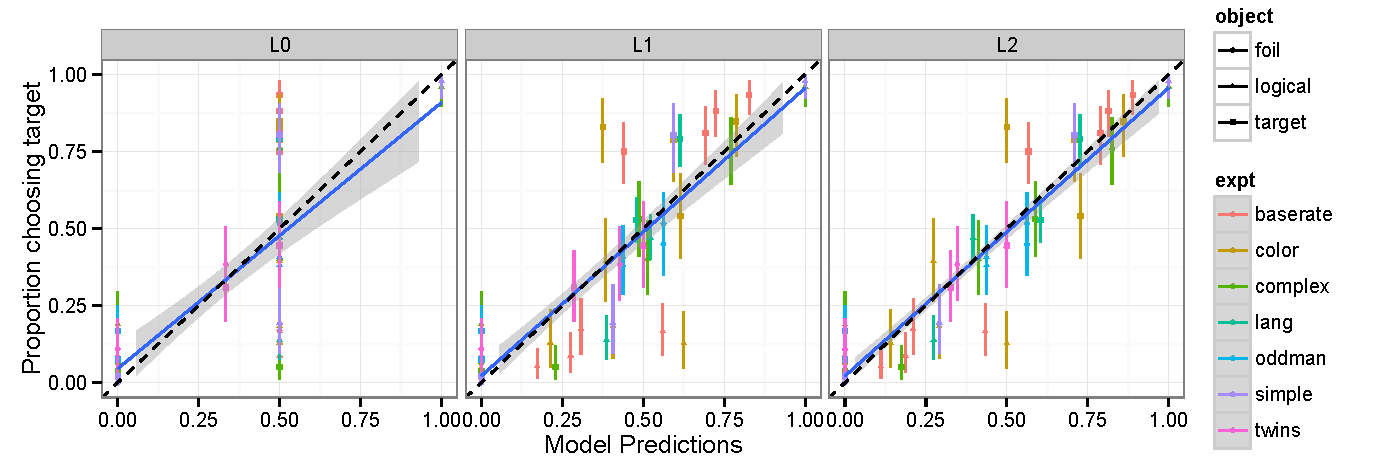
\includegraphics[width=6in]{../plots/models-1.pdf}
  \caption{\label{fig:models-2} Full model fit to data for $L_0$, $L_1$, and $L_2$. Each point represents proportions choosing a particular target object in an experimental condition. The diagonal dashed line shows perfect fit, and the blue solid line shows a line of best fit with 95\% confidence intervals.}
\end{figure}

In our first analysis, we 


\subsection{Identifiability}

%%% Local Variables: 
%%% TeX-master: "pragmods"
%%% End:


\section{General Discussion}
\label{sec:discussion}


\subsection{Other work using RSA and variants}

Epistemic inferences \cite{goodman2013}

Affective \cite{kao2014}


Quantifiers \cite{franke2013}


Embedded implicature \cite{pottsunderreview}

\subsection{Limitations}




\newpage

\bibliographystyle{apacite}
\bibliography{pragmods}

\newpage

\theappendix

\section{Equivalences}

The model we describe above has as its special case several previous systems; in what follows we show these equivalences, as they motivate our experiment below.

\subsection{J\"ager (to appear)}

The system described here is a restatement and generalization of the Iterated Best Response model described in J\"aeger's work \cite{jaegerinpress}. That work notates $S(C^T)$ as $\sigma$, and proposes an algorithm in which recursive applications of $L^*$ and $S^*$ are made until $X = L(S(X))$. 

\subsection{Frank \& Goodman (2012)}

In recent work, Frank \& Goodman \cite{frank2012} described a utility-theoretic derivation of a similar framework. They start with the idea that speakers choose messages relative to their utility with respect to the number of bits of information they would send to a simple, truth-functional listener; this formulation reduced to

\begin{equation}
P(w|r_S,C) = \frac{|w|^{-1}}{\displaystyle \sum_{w' \in W} {|w'|^{-1}}},
\end{equation}

where $|w|$ indicated the number of objects to which $w$ could refer. The associated listener probability was given by Bayesian inference from the speaker's likelihood and a prior term $P(r_S)$:

\begin{equation}
\label{eq:fg}
% P(r_S | w, C) \propto P(w | r_S, C) P(r_S).
P(r_S | w, C) 
= \frac{P(w | r_S, C) P(r_S)}{\displaystyle \sum_{r' \in C}{P(w | r', C) P(r')}} =
\frac{\frac{\displaystyle |w|^{-1}}{\displaystyle \sum_{w' \in W} {|w'|^{-1}}}P(r_S)}{\displaystyle \sum_{r' \in C}{\frac{|w|^{-1}}{\displaystyle \sum_{w' \in W} {|w'|^{-1}}}P(r')}}.
% \frac{|w|^{-1}}{\displaystyle \sum_{w' \in W} {|w'|^{-1}}}
\end{equation}

Working from our definitions, this formulation is equivalent to $L_B(S(L(C)))$. We can rewrite $L(C_{o,w})$ using the same notation as above, with $|w|$ as the number of objects to which a word refers. This allows us to write 

\begin{eqnarray*}
% L(C_{o,w}) = \frac{C_{o,w}}{\displaystyle\sum_{o' \in C} C_{o',w}} = |w|^{-1} \\
S(L(C_{o,w})) &=& \frac{|w|^{-1}}{\displaystyle \sum_{w' \in V(C)} |w|^{-1}} \mbox{, and} \\
L_B(S(L(C_{w,o}))) &=& \frac{ \frac{\displaystyle |w|^{-1}}{\displaystyle \sum_{w' \in V(C)} |w|^{-1}}P(o)}{\displaystyle\sum_{o' \in C}  \frac{|w|^{-1}}{\displaystyle \sum_{w' \in V(C)} |w|^{-1}}P(o')},
\end{eqnarray*}

which is equivalent to Equation \ref{eq:fg}.

\subsection{Other work}

Golland, Liang, and Klein \cite{golland2010} describe a similar system based on \cite{jaegerinpress}, in which they call $S(C^T)$ the ``reflex speaker'' and $S(L(C))$ the ``reasoned speaker.'' Benz \cite{benz2005b} describes a game-theoretic system that is similar to $S(L(C))$. 

\subsection{An example}

% \begin{figure}[t]
%   \begin{center} 
%     \includegraphics[width=4.5in]{figures/bugs.jpg} 
%     \caption{\label{fig:ex} An example stimulus for our 3 objects, 3 features experiment. Inferring that ``tail'' referred to C is a depth-0 computation, inferring that ``feet'' referred to A is a depth-1 computation, and inferring that ``horns'' referred to B is a depth-2 computation.} 
%   \end{center} 
% \end{figure}

We work through an example computation on the stimulus shown in Figure \ref{fig:ex}, using the J\"ager \cite{jaegerinpress} version of the model described above (for simplicity and finite convergence): $L^*(S^*(L^*(S(C^T))))$. The object by feature matrix $C$ has as its columns the messages ``tail,'' ``horns,'' and ``feet'' and the objects A, B, and C as its rows.:

\begin{equation}
C= \left(
    \begin{array}{ccc}
      0 & 0 & 1 \\
      0 & 1 & 1\\
      1 & 1 & 0 
    \end{array} 
  \right)
\end{equation}

The corresponding speaker matrix $S(C^T)$ is inverted, with messages as rows and objects as columns: 

\begin{equation}
E = \left(
    \begin{array}{ccc}
      0 & 0 & 1 \\
      0 & .5 & .5\\
      .5 & .5 & 0 
    \end{array} 
  \right)
\end{equation}

It is already clear that ``tail'' is true only of object C, thus the interpretation of ``tail'' reaches depth 0. Now we perform a set of renormalizations to lead to the next level of recursion:

\begin{equation}
L^*(S(C^T)) = \left(
    \begin{array}{ccc}
      0 & 0 & 1 \\
      0 & .5 & .5\\
      1 & 0 & 0 
    \end{array} 
  \right)
\end{equation}

Now, at depth 1, the message ``feet'' is found to refer to object A. A final round of recursion leads to depth 2, where ``horns'' is found to refer to object B:

\begin{equation}
L^*(S^*(L^*(S(C^T)))) = \left(
    \begin{array}{ccc}
      0 & 0 & 1 \\
      0 & 1 & 0\\
      1 & 0 & 0 
    \end{array} 
  \right)
\end{equation}

We now say that the model has ``converged''---that is, further iteration will not lead to changes in state.



\section{Appendix B: An alternative, matrix-based presentation}
\label{app:matrix}

This probabilistic notation emphasizes individual interpretation probabilities and is consistent with previous presentations of the RSA model.


The first function, $S(x)$, is the speaker function, which captures the intuition that the speaker chooses the best word to describe a particular object (from those that are available in the vocabulary). $S(x)$ takes an object-word pair from a matrix $X$ and returns the probability of speaking this word, normalized over the other possible words. ($x$ here gives some base probabilities over terms applying to objects.)

\begin{equation}
S(x_{o,w}) = \frac{x_{o,w}}{\displaystyle \sum_{w' \in V(C)} x_{o,w'}}
\end{equation}

The second function, $L(x)$, is the listener function, which is a complement to the speaker function; for a particular object word pair, it returns the probability of that object, given the word. 
% The listener function contains one other constraint, which is that listeners are assumed to consider only true statements. To enforce this constraint, elements are multiplied by $E$, the extension matrix (which is uniform over those objects to which a word refers). 

\begin{equation}
L(x_{o,w}) = \frac{x_{o,w}}{\displaystyle\sum_{o' \in C} x_{o',w} } %C_{o',w} C_{o,w}
\end{equation}

We also define variants on these functions. The first variant is greedy listeners and speakers $L^*$ and $S^*$, where

\begin{equation}
L(x_{o,w}) = 
\begin{cases}
1 & \mbox{if } o = \displaystyle \argmax_{o} \frac{x_{o,w} C_{o,w}}{\displaystyle\sum_{o' \in C} x_{o',w} C_{o',w}} \\
0 & \mbox{otherwise}.
\end{cases}
\end{equation}

and $S^*$ is defined similarly. 

Second, we define a Bayesian listener $L_B$ who considers the prior probability $P(o)$ of each object in making a selection. 

\begin{equation}
L_B(x_{o,w}) = \frac{x_{o,w} C_{o,w} P(o)}{\displaystyle\sum_{o' \in C} x_{o',w} C_{o',w} P(o')}
\end{equation}

We could also introduce a Bayesian speaker $S_B$ who considers a prior probability over words, but all words were considered equiprobable in our simulations and so we do not pursue this possibility in the current work. (Although they are not referred to this way, this definition highlights that $L$ and $S$ represent a maximum likelihood listener and speaker). 

For convenience, we assume that these functions can be applied over full matrices; hence we can write $L(X)$ to indicate the matrix that is produced by applying $L$ to all the elements of $X$. We can thus write statements like $L(S(C))$ or $L^*(S(L(C)))$ to indicate the recursive application of these functions to a context.\footnote{Note that when applied to matrices, $S(X)$ takes $C^T$ as its input, rather than C.}



% We also treat the contextual salience distribution $\sigma$ as a special starting point, where we assume that it can be tiled (FIXME) uniformly over words so that we can write $L(\sigma)$ to produce a depth-1 computation that starts from the contextual salience distribution. 

% In previous literature, these functions have been assumed to operate deterministically, by greedily choosing the highest probability word or object, respectively. We notate these greedy versions of the functions by $L^*(\rho)$ and $S^*(\rho)$.

\end{document}

